\documentclass{chi2009}
\usepackage{times}
\usepackage{url}
\usepackage{graphics}
\usepackage{color}
\usepackage[pdftex]{hyperref}
\usepackage{graphicx}
\usepackage{tabularx}
\usepackage{booktabs}

\newcommand{\docTitle}{Improving Usability of the Linux Kernel Configuration Tools}
\newcommand{\docKeywords}{usability, linux, kernel, configuration}

\hypersetup{%
pdftitle={\docTitle},
pdfauthor={Kacper Bak},
pdfkeywords={\docKeywords},
bookmarksnumbered,
pdfstartview={FitH},
colorlinks,
citecolor=black,
filecolor=black,
linkcolor=black,
urlcolor=black,
breaklinks=true,
}
\newcommand{\comment}[1]{}
\definecolor{Orange}{rgb}{1,0.5,0}
\newcommand{\todo}[1]{\textsf{\textbf{\textcolor{Orange}{[[#1]]}}}}
\newcolumntype{S}{>{\centering\arraybackslash} m{.4\linewidth} }

%
%  Convenience commands for references
%
\newcommand{\secref}[1]{Sect.~\ref{sec:#1}}
\newcommand{\tabref}[1]{Table~\ref{tab:#1}}
\newcommand{\figref}[1]{Fig.\,\ref{fig:#1}}
\newcommand{\Figref}[1]{Figure\,\ref{fig:#1}}
\newcommand{\eqaref}[1]{equation~\eqref{eq:#1}}
\newcommand{\defref}[1]{Definition~\eqref{def:#1}}
\newcommand{\lemref}[1]{Lemma~\eqref{lem:#1}}
\looseness=-1

\pagenumbering{arabic}  % Arabic page numbers for submission.  Remove this line to eliminate page numbers for the camera ready copy

\begin{document}
% to make various LaTeX processors do the right thing with page size
\special{papersize=8.5in,11in}
\setlength{\paperheight}{11in}
\setlength{\paperwidth}{8.5in}
\setlength{\pdfpageheight}{\paperheight}
\setlength{\pdfpagewidth}{\paperwidth}

% use this command to override the default ACM copyright statement 
% (e.g. for preprints). Remove for camera ready copy.
\toappear{Submitted for CS 889 - Open Source Usability.}

\title{\docTitle}
\numberofauthors{2}
\author{
  \alignauthor Kacper Bak\\
    \affaddr{Generative Software Development Lab}\\
    \affaddr{University of Waterloo, Canada}\\
    \email{kbak@gsd.uwaterloo.ca}
  \alignauthor Karim Ali\\
    \affaddr{PLG Group}\\
    \affaddr{University of Waterloo, Canada}\\
    \email{karim@uwaterloo.ca}
}

\maketitle

\begin{abstract}
Tailoring a Linux kernel to one's needs has been one of the most cumbersome tasks a GNU/Linux user can do. There have been many attempts to overcome this problem by introducing smarter configuration tools. Those tools, however, still lack some important features, which discourages users from using them. In this project, we addressed the problem of usability of the Linux kernel configuration tools. We identified the major usability issues with current tools, proposed a better user interface and evaluated it on a group of Linux enthusiasts.
\end{abstract}

\keywords{\docKeywords} 

\category{H.5.2}{Information Interfaces and Presentation}{Miscellaneous}%[Optional sub-category]

\section{Introduction}

GNU/Linux is a free operating system with Linux as its kernel. The Linux kernel\footnote{Available at: \url{http://www.kernel.org/}} is a mature and very complex piece of software. It has been developed by thousands of programmers led by Linus Torvalds since 1991. The kernel supports a variety of computer architectures, network protocols, thousands of drivers, and many debugging options.

Structure of the kernel is very modular, so that each user can tailor it to her particular needs and specific hardware. Recent research \cite{she:kernel:2010} has shown that the whole kernel is composed of almost 5500 features, of which 89\% are user-selectable. Thus, the variation space is huge and the configuration process requires a broad computer knowledge. Users can configure kernel either by manually editing the \textsf{.config} file or by using some configuration tool (i.e. \textsf{menuconfig, xconfig, gconfig}). The first option is discouraged, because it is very error-prone due to lack of automated constraint validation/propagation. Using a configurator is a better solution, but it is still a laborious process.

Existing configuration tools have been evolving for over a decade, but the progress is reasonably slow compared to other parts of the kernel. Usability seems to have low priority on developers' task lists. To address this issue, we started a course project aimed at making the configuration process easier and more intuitive for Linux enthusiasts. In the project we investigated current configuration tools, identified major usability issues, proposed alternative designs, chose the most promising one and evaluated it on users. General reactions were positive and participants said the new tool was an improvement over the standard tools. We believe that our findings will help in creating better configuration applications not only for the Linux kernel, but also for other kinds of variability models.

The paper is organized as follows. We describe the problem domain and results of our initial study of standard tools in \secref{problem}. We explain how we reached the new design and how it compares to \textsf{xconfig} in \secref{lkc}. We then present evaluation of the new tool in \secref{evaluation}. We discuss future work in \secref{futurework}. After presenting related work in \secref{relatedwork}, we conclude in \secref{conclusion}.

\section{Problem}\label{sec:problem}

% motivation
There are several reasons why people configure operating system kernels. Usually they want to customize kernels to specific hardware or to particular needs. This scenario is very common in embedded systems, such as network routers. By carefully selecting options, one can improve system stability or functionality. Although many configuration options are related with hardware and device drivers, there is also a large group of options that change the way operating system works. A good example is ``preemptible scheduler'' that makes Linux a soft real-time operating system. Such a scheduler is desirable for digital signal processing, e.g. for recording and transforming signal from the guitar.

Majority of users configure kernels without even realizing this fact. We distinguish two types of kernel configuration: static and dynamic. In the former method software is customized before compilation, so that only chosen pieces of code are compiled. It results in a smaller program footprint and faster compilation. On the other hand, later reconfiguration requires more effort, because any additional piece of software has to be compiled separately. In many modern distributions users are provided with fully functional kernels, and they do not have to compile themselves. Instead, they dynamically customize the software, by loading relevant modules. The disadvantage of the second method is that preparing such a big kernel takes a lot of time and resources. Furthermore, it is infeasible to apply it to embedded systems.

% current sw
Regardless of configuration type, there is still need to customize the software. Although this task can be done manually, users prefer to use automated and intuitive tools, that could guarantee that the system works properly. Unfortunately, the software currently used for kernel configuration is neither fully automated, nor easy to use. In addition, static and dynamic configuration are two separate mechanisms and are supported by completely different programs. Static configuration is done by the Linux Kernel Configurator, while dynamic configuration is about adding or removing compiled modules. In our opinion the two worlds can be merged by providing a unified user interface.

Linux kernel configurators are targeted to advanced users. Some kernel developers expressed opinion \cite{kernel:aunt:2002} that kernel should be configured only by experienced users. While this statement might be true, there are still lots of Linux novice users who want to learn how to configure kernel or need to compile/load a particular driver. As of now, there are millions of web pages describing how to configure and compile the Linux kernel. Novice users are often overwhelmed by the number of available options and required knowledge. To understand challenges of configuration, we carried out an initial study on a group of Linux users.

% initial study
In the study six participants were asked to statically configure the Linux kernel for a popular laptop for typical home or office use. They used the standard \textsf{xconfig} tool that comes with the Linux kernel. It presented a list of options in a tree structure composed of categories and options. A person succeeded if the new kernel was ready to play music and movies, connect to Ethernet, use WiFi, memory cards, USB devices, Bluetooth, CD/DVD. This scenario seemed rather common, because in many Linux distributions users have to fine-tune their configurations to make the whole system work as expected. None of the subjects succeeded with the task without further help. We observed many problems that people faced during the configuration process. It is worth noting, that our participants had previous experience with Linux and claimed to be advanced computer users. During the study, we were also interested in how they used \textsf{xconfig}, and how people configure software in general. Our findings are summarized in several categories:

\begin{description}
  \item[Menu hierarchy]
All participants had problems with selecting drivers for laptop's hardware. First of all, the tool showed the whole hierarchy, and people said they were overwhelmed by thousands of options. Several of them started with collapsing all menus, so that only top-level categories were visible. Furthermore, the tree/sub-tree relationship was confusing. It was unclear whether selection of parent option implies selection of required functionality or additional suboptions should be selected as well. To some, even such a basic thing as checking an option was confusing. Besides familiar empty and filled checkbox, the tool showed a box with dot inside. It meant that the option will be compiled, but as a dynamically loadable module.

  \item[Option names and descriptions]
Cryptic names were another source of problems. The existing infrastructure use names that make sense to programmers and kernel hackers, but are hard to understand for less experienced users. Unfortunately, descriptions were not very helpful, since they often explained implementation details instead of end-user functionality. Participants expected to see what selecting an option means for them and whether the device driver is appropriate for their hardware. In many cases their expectations turned out to be too high.

  \item[Searching]
Huge hierarchy of options and cryptic names make it very hard to find a particular feature. All participants used search in \textsf{xconfig}. Searching worked very poorly, since feature descriptions were skipped by the tool. People expressed their frustration and often used Google to match modules with hardware, and later select the module in \textsf{xconfig}. Google was also used to find a list of drivers required by the laptop. For all users, querying a web search engine was easier than running system tools to discover hardware devices.

  \item[Configuration]
We carefully observed how users used current tools to configure a large piece of software. Most of them were jumping between different categories as they tried to locate modules. One person, who had experience with kernel configuration tools, started \textsf{menuconfig} program, which performs wizard-like configuration. The problem with this tool was that the user could not jump to other categories, but had to answer many irrelevant questions. After a while, the participant switched to \textsf{xconfig}. Users had problems with selecting appropriate device drivers. When users were unsure about which module to choose, because 2-3 modules seemed similar, they checked them all. 
\end{description}

% conclusions

The initial study was a necessary step to discover user expectations and needs. It led us to the following conclusions:
\begin{enumerate}
\item Menu hierarchy should be as simple as possible. There are far too many options that could be reduced automatically if the configuration tool targeted specific user group and had good reasoning capabilities.
\item Feature names and descriptions should reflect end-user functionality instead of low-level details.
\item Powerful searching capabilities are crucial as the number of configuration options grows.
\item Automatic hardware detection and kernel autoconfiguration is important, since majority of kernel options is related to hardware drivers.
\end{enumerate}

The aforementioned problems can be fixed by improving application's backend and creating a more intuitive user interface. Our project focused on constructing a GUI that would be intuitive, simple and targeted to specific group of users.

\section{Linux Kernel Configuration Tool}\label{sec:lkc}
% target group

To design such configuration tool, we first set our target group to be less experienced Linux users. In other words, we are building this tool for novice and
intermediate Linux users to allow them to to configure a Linux kernel withouth burdening them with many of the unncessary details involved during such process.
We started the design process of our Linux Kernel Configuration Tool (lkc tool) by designing several mockups that have our vision for the tool. Initially, we
thought that once the tool is started, it should first fetch the current Linux kernel configuration, then detect the currently connected hardware. A dialog box
(splash screen) should be shown to the user at that time to show the progress of these processes. Figure \ref{fig:splash} shows four different mockups for that
dialog box. 

% rationale for the design

\begin{figure*}[!t]
 \centering
\begin{tabular}{SS}
 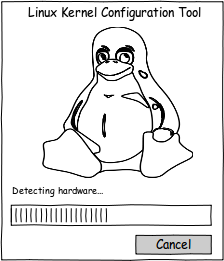
\includegraphics[scale=0.5,keepaspectratio=true]{figs/splash-big} & 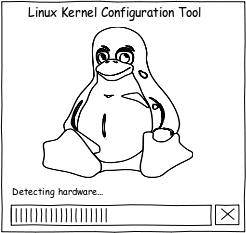
\includegraphics[scale=0.5,keepaspectratio=true]{figs/splash-bigico} \\
 (a) & (b) \\
 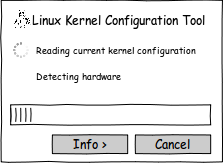
\includegraphics[scale=0.5,keepaspectratio=true]{figs/splash-readingcurrent} &
 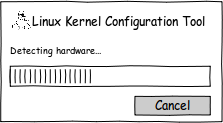
\includegraphics[scale=0.5,keepaspectratio=true]{figs/splash-standard} \\
 (c) & (d) \\
\end{tabular}
\caption{Splash screen design mockups}
\label{fig:splash}
\end{figure*}

We decided to do a second user study that included six participants. The aim of this study was to show the participants those designs and get feedback from
them regarding what aspects in those designs were appealing to them, and what were not. That study led us to draw the following conclusions:
\begin{enumerate}
 \item Users always liked to know what is going on. In other words, they did care about getting more information about what the tool is doing while the progress
bars are being filled up.
 \item The fact that users appreciate access to more information does not mean they appreciate that such information should be displayed by default, only when
requested.
 \item It is highly desirable to have the tool report to them any crashes that occur during the hardware detection process.
\end{enumerate}

Consequently, we settled down on the design shown in Figure \ref{fig:splash-final} for our splash screen. In the final design of the splash screen, the user
will be asked a question whether she wants to detect the current hardware or not. If she answered yes to that question, she will be presented with the dialog
shown in Figure \ref{fig:splash-final}a. The list of tasks along with the progress bar gives the user an idea about the task that the tool is currently doing.
If the user would like to get more information, she can click on the \textquotedblleft Information \textquotedblright button. The user will then be presented
by a scrollable window that shows the current action (e.g. detecting device ... dev 40). This window is hidden by default so that it does not get into the way
of the user while using the tool. In case of a crash occured, this window will show more information to the user about what are the possible causes of the crash
and what the progress of the tool so far.

\begin{figure*}[!t]
 \centering
\begin{tabular}{SS}
 \begin{tabular}{c}
  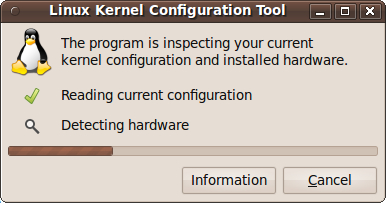
\includegraphics[scale=0.5,keepaspectratio=true]{figs/splash-final1} \\
  (a) \\
 \end{tabular}
  & 
\begin{tabular}{c}
  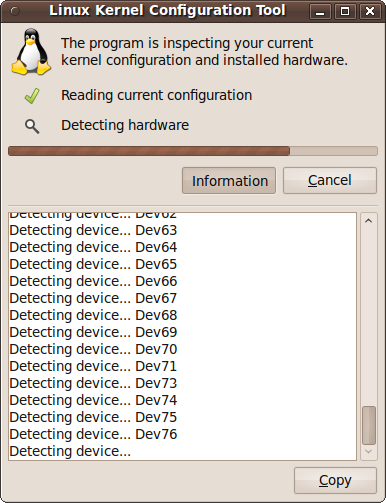
\includegraphics[scale=0.5,keepaspectratio=true]{figs/splash-final2} \\
  (b) \\
 \end{tabular}
\end{tabular}
\caption{Final splash screen design}
\label{fig:splash-final}
\end{figure*}

% xconfig vs lkc

% scalability

% implementation

\section{Evaluation}\label{sec:evaluation}

% participants characterization

\subsection{Threats to Validity}

\paragraph{External Validity}

\paragraph{Internal Validity}

\section{Future Work}\label{sec:futurework}

% \section{Future Work} - we'll place this section in the final report
% \todo{what do you think about creating a graphical tool that goes with you step by step and configures a kernel? basically you answer some questions, press next, and finally click install to install the new kernel. It might be appreciated by beginners. Is it too simplistic? would it be useful? it improves usability, but are there many users who need such a limited tool?}

% backends

\section{Related Work}\label{sec:relatedwork}
% literature review

All the Linux kernel configuration tools are front-ends built on top of a single engine called Linux Kernel Configurator (LKC). LKC analyzes kernel variability and supports users during the configuration stage. LKC uses internally the KConfig language to represent variability and dependencies among features. As several researchers \cite{sincero:lkc:2008,she:kernel:2010} showed, there is a direct correspondence between well-understood feature models and practically crafted variability model used by the Linux kernel. In contrast with formal feature models, LKC is not supported by any formal reasoning engine (e.g. SAT-solver). This is a serious problem, because users can unconsciously create wrong configurations while having no clue why a particular configuration does not work. The Linux kernel community can benefit from adopting well-researched feature models, and make their tools more reliable and usable.

\textit{eCos}~\cite{veer:ecos:2000} is an open source real-time operating system. It was designed to be configurable and run on a wide variety of hardware platforms. Similarly to the Linux kernel, eCos comes with configuration tools. The eCos configurator, is much more advanced, and arguably better-thought, since it can detect conflicting options and guide users to resolve them. The eCos Configuration Tool has many features, but presents them in a single tree hierarchy. In comparison with our tool, eCos features are often low-level and very technical. The eCos Configuration Tool also does not offer any wizard, so users must have expertise if they want to skip irrelevant categories.

Hardware autodetection and kernel configuration is a recurring problem \cite{debian:config:2010,soft32:config:2007}. Many users complain about the lack of it. The situation is slowly improving as developers added the \textsf{localmodconfig} \footnote{More info at: \url{http://bit.ly/cPgq8R}} target to Linux-2.6.32. The command detects current kernel configuration and applies the same options to the new kernel. It is a step ahead, but the tool is very simplistic and assumes that all the required modules are already loaded. For example, if a computer has built-in Bluetooth, but the module is not loaded, the new kernel will not support the Bluetooth device. Furthermore, the autoconfiguration script offers a very coarse level of options granularity, e.g. if a computer has one sound card, such as Intel HD Audio, the script will select all available sound card drivers and all Intel HD Audio modules. The autoconfiguration tool reads configuration of the running kernel instead of detecting the actual hardware, e.g. for a laptop with the Core Duo 2 processor, it selected 686 processor in the new kernel, because that processor is selected in the running kernel.

System configuration is a necessary, but uneasy process. Our tool tried to simplify it by asking as few questions as possible and targeting specific group of users. The same direction is suggested in \cite{spillers:config:2010}. The author goes even further saying that software shall configure itself automatically. We agree with many points from the post, but making a configuration-free kernel on any platform seems rather impossible due to extra knowledge that is not included in configurators.

Improvements of kernel configuration tools were already introduced in 2002 when Eric S. Raymond presented the CML2 configuration system \cite{raymond:cml2:2000}. It allowed for effective reasoning on kernel feature model and also provided progressive-disclosure. There was a long debate and flame war about using that system \cite{kerneltrap:linux:2002}. Finally, it was rejected for various reasons, such as Eric S. Raymond's attitude, Python dependency, complexity, radically new design. Many developers preferred to introduce gradual updates instead of applying one big patch.

Debian GNU/Linux device driver check \& report~\cite{muto:check:2010} is an interesting project that helps with matching kernel modules with hardware. It reads output of \textsf{lspci} command, and then outputs driver's name. The project is in fact a big database that stores user's knowledge about the hardware. It could be utilized by the configurator to automatically select relevant modules if autodetection fails. Currently, the database aggregates only information about PCI devices, and does not support ISA, USB, IEEE1394 or other hardware.

% OSS usability
Free and Open Source Software usability has recently got attention from both academia and FOSS community. Several researchers \cite{nichols:usability:2003,andreasen:usability:2006} tried to understand why FOSS developers traditionally gave low priority to usability issues. Other works studied particular projects, such as Apache \cite{mockus:apache:2000} or Mozilla \cite{mockus:mozilla:2002} to learn about social interactions, FOSS culture and the way the software is developed. Cooperation of the two communities allows usability people to understand attitudes of FOSS developers. FOSS community, on the other hand, benefits from transferring usability knowledge and evaluation techniques.

\section{Conclusion}\label{sec:conclusion}

\bibliographystyle{abbrv}
\bibliography{doc}

\end{document}
